\section{Chapter 11}
\subsection{11.1}
%TODO: 11.1 – 2, 4, 6, 10, 18, 20
\begin{itemize}
    \item[2.] Which of these graphs are trees? \vspace{1mm}\\
          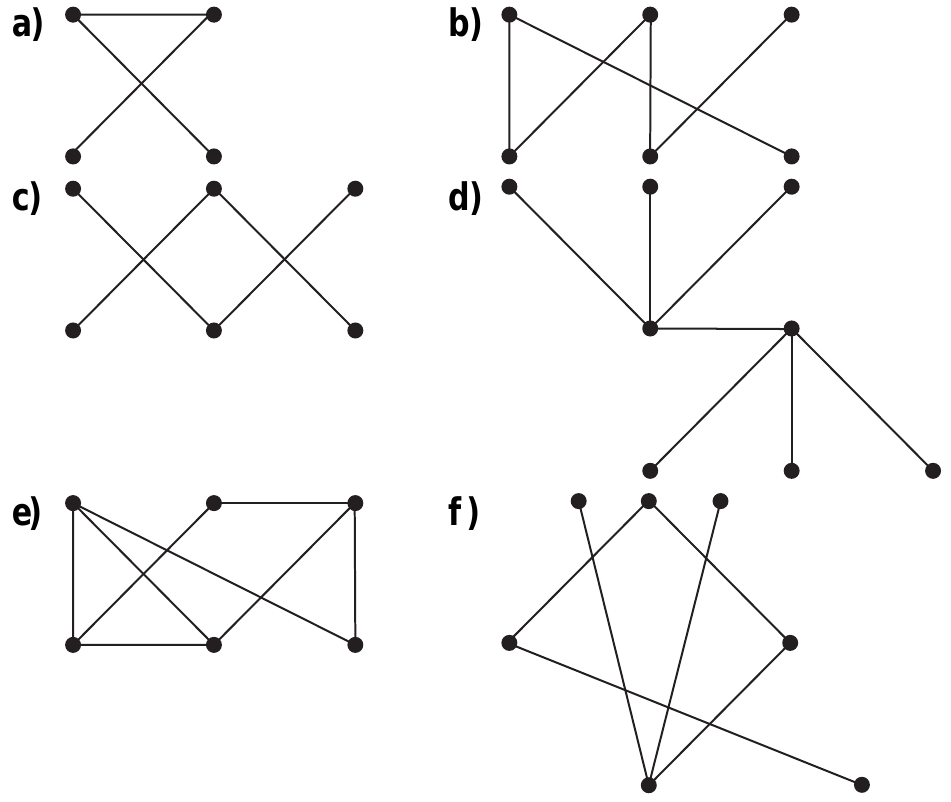
\includegraphics[scale = 0.4]{img/11_1_2_graphs.png} \\
          \answer
          \begin{tasks}(2)
              \task Tree
              \task Tree
              \task Not a tree
              \task Tree
              \task Not a tree
              \task Tree
          \end{tasks}
          \newpage
    \item[4.] Answer these questions about the rooted tree illustrated. \\
          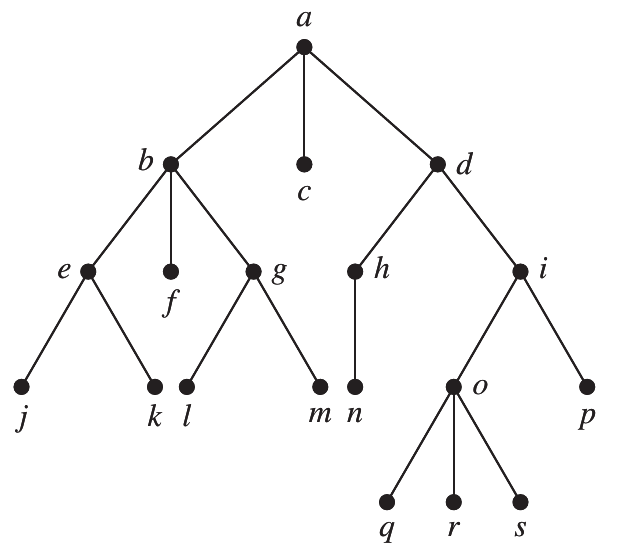
\includegraphics[scale = 0.5]{img/11_1_4_graph.png} \\
          \begin{enumerate}[a.]
              \item Which vertex is the root?
              \item Which vertices are internal?
              \item Which vertices are leaves?
              \item Which vertices are children of j ?
              \item Which vertex is the parent of h?
              \item Which vertices are siblings of o?
              \item Which vertices are ancestors of m?
              \item Which vertices are descendants of b?
          \end{enumerate}
          \answer
          \begin{enumerate}[a.]
              \item $a$
              \item $a, b, d, e, g, h, i, o$
              \item $c, f, j, k, l, m, n, p, q, r, s$
              \item $j$ has no children.
              \item $d$
              \item $p$
              \item $g, b, a$
              \item $e, f, g, j, k, l, m$
          \end{enumerate}

    \item[6.]  Is the rooted tree in Exercise 4 a full m-ary tree for some
          positive integer m? \\
          \answer \\
          No, it's not a full m-ary tree because there are some internal nodes who
          have a different ammount of children. For example, $b$ has 3 children but "i"
          only has 2.

    \item[10.]  Draw the subtree of the tree in Exercise 4 that is rooted
          at
          \begin{tasks}(3)
              \task a.
              \task c.
              \task e.
          \end{tasks}
          \answer
          \begin{tasks}(3)
              \task \text{}\\
              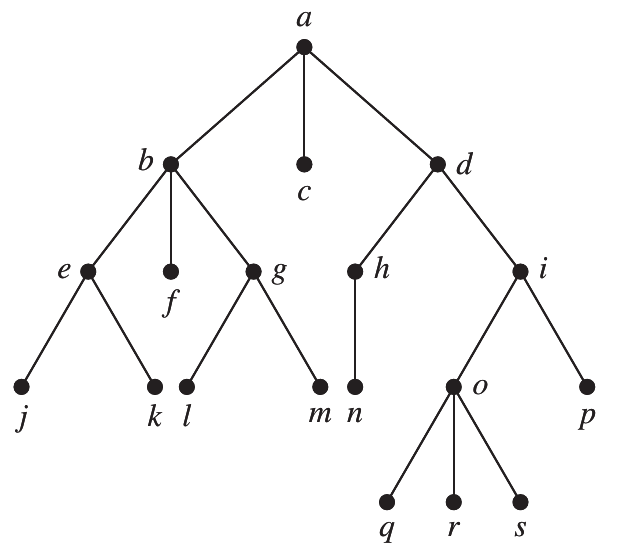
\includegraphics[scale = 0.35]{img/11_1_4_graph.png}

              \task \text{}\\
              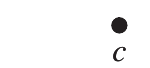
\includegraphics[scale = 0.5]{img/11_1_10b_graph.png}

              \task \text{}\\
              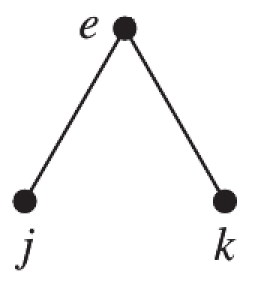
\includegraphics[scale = 0.4]{img/11_1_10c_graph.png}
          \end{tasks}

    \item[18.] How many vertices does a full 5-ary tree with 100 internal
          vertices have? \\
          \answer \\
          $n = mi + 1 = 5 \cdot 100 + 1 = 501$ vertices.

    \item[20.]  How many leaves does a full 3-ary tree with 100 vertices
          have? \\
          \answer \\
          $l = n - (n-1)/m = 100 - 99/3 = 67$ leaves.
\end{itemize}

\subsection{11.3}
%TODO: 11.3 – 8, 12, 14, 16, 22, 24
\begin{itemize}
    \item[8.] Determine the order in which a preorder
          traversal visits the vertices of the given ordered rooted tree. \\
          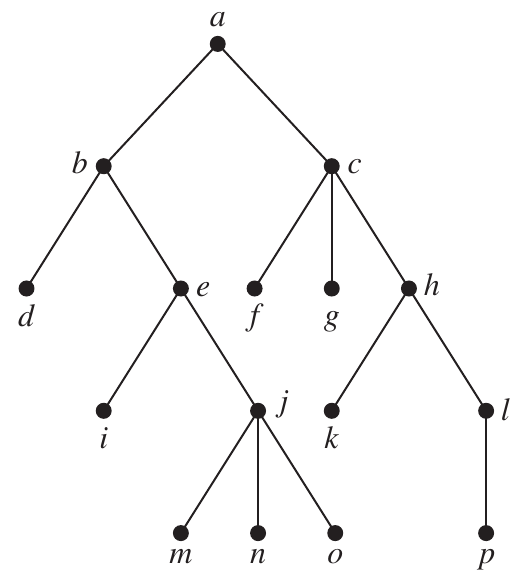
\includegraphics[scale=0.6]{img/11_3_8_tree.png} \\
          \answer \\
          \textit{a, b, d, e, i, j, m, n, o, c, f, g, h, k, l, p}

 \newpage

    \item[12.]  In which order are the vertices of this ordered rooted tree
          visited using an inorder traversal? \\
          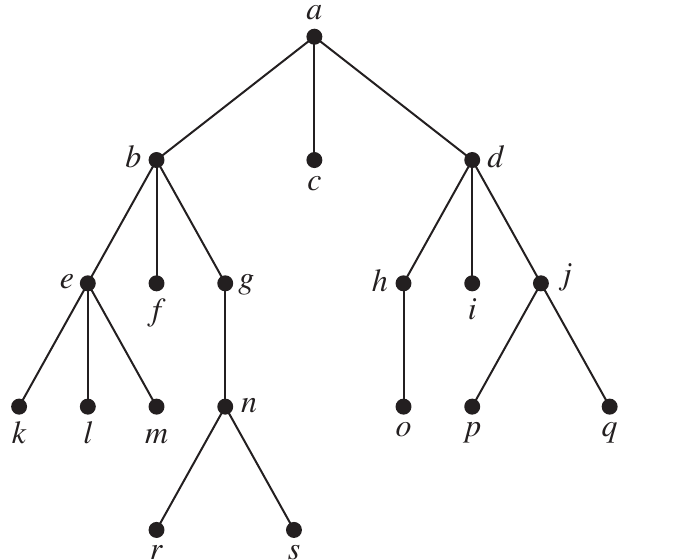
\includegraphics[scale=0.6]{img/11_3_12_tree.png} \\
          \answer \\
         \textit{k, e, l, m, b, f, r, n, s, g, a, c, o, h, d, i, p, j, q}

    \item[14.] In which order are the vertices of the ordered rooted tree
in Exercise 8 visited using a postorder traversal?\\
\answer \\
\textit{d, i, m, n, o, j, e, b, f, g, k, p, l, h, c, a}

\item[16.] Represent the expression
 $((x + 2) \uparrow 3) \cdot (y -(3 + x)) - 5$ using a binary tree.



\end{itemize}

\subsection{11.4}
%TODO: 11.4 – 4, 8, 10, 14, 16